\documentclass[../diplomski_rad.tex]{subfiles}

\begin{document}


\sloppy

\justifying

U ovom poglavlju iznesen je proces razvoja programske potpore za ranije opisani nosivi ugradbeni sustav. 
Programska potpora za korišteni mikrokontroler STM32WB55VGY razvijena je pomoću operacijskog sustava 
za ugradbena računala Zephyr.

Za utakanje programske potpore na razvijenu pločicu i testiranje sustava korišten je ST-LINK/V2 programator \cite{stm32programator}. 
Progamator se na mikrokontroler spaja putem SWD sučelja (engl. \textit{Serial Wire Debug}). 
Kao razvojno okruženje korišten je Visual Studio Code, a kontrola verzija praćena je sustavom git.

Ovaj integrirani pristup omogućio je efikasno razvijanje i upravljanje programskom podrškom za STM32 mikrokontroler, 
uz korištenje popularnih alata i tehnologija. 
U nastavku će se detaljno opisati proces razvoja, implementacija, te testiranja programske potpore, 
uz naglasak na integraciju sa Zephyr operacijskim sustavom.

\section{Programiranje mrežnog procesora ARM Cortex-M0+}

STMicroelectronics pruža već gotove binarne datoteke \cite{kodovi_M0} koje sadrže kod komunikacijskog stoga. 
Postoje različite verzije komunikacijskog stoga s obzirom na primjenu te je samo potrebno pronaći odgovarajuću 
binarnu datoteku i učitati ju na jezgru ARM Cortex-M0+.

Za potrebe ovog projekta odabrana je datoteka \textit{stm32wb5x\_BLE\_HCILayer\_extended\_fw.bin} jer je kompatibilna sa 
korištenim operacijskim sustavom Zephyr. Datoteka je učitana na procesor pomoću programa STM32CubeProgrammer v2.15.0 
koji u sebi ima ugrađenu podršku za ažuriranje koda komunikacijskog stoga. 

\section{Operacijski sustav za rad u stvarnom vremenu Zephyr}

Operacijski sustav Zephyr predstavlja sofisticiranu platformu optimiziranu za ugradbena računala, 
pružajući niz prednosti koje ga čine idealnim izborom za širok spektar aplikacija. 
Njegova modularna arhitektura omogućuje prilagodbu specifičnim potrebama svakog uređaja, 
dok istovremeno osigurava visoku razinu pouzdanosti i performansi.

Glavna prednost Zephyra u odnosu na druge operacijske sustave za rad u stvarnom vremenu je njegova prilagodljivost 
na razlčite arhitekture mikrokonrolera. 
Drugim rječima, isti kod, uz minimalnu promjenu konfiguracijkih datoteka, možemo koristit na potpuno 
različitim porodicama mikrokontrolera. Iz tog razloga se prilikom razvoja ugradbenog uređaja programska potpora može razvijati 
i dok sklopovlje još nije dostupno.
Također, u sklopu Zepyhr-a već su uključeni brojni upravljački programi za često korištene periferijalne 
uređaje i senzore. Iz svega navedeno vidljivo je kako korištenje operacijskog sustava Zephyr u konačnici 
znatno ubrzava razvoj uređaja.

Glavne dvije datoteke za konfiguraciju Zephyr projekta su \texttt{.conf} te \texttt{.dts} datoteke. 
\texttt{.dts} datoteka (engl. \textit{dts, device tree structure}) datoteka je koja opisuje sklopovlje koje se programira. 
U njoj se specifiraju pinovi na koje su spojene korištene periferije mikrokontrolera. 
Prilikom promjene sklopovlja samo je potrebno promjeniti ovu datoteku. U \texttt{.conf} datoteci specificiraju se 
konfiguracijske konstante i uključuje programska potpora za različite periferije.

\section{Opis upravljačkog programa za MAX30009}

Integrirano sučelje za mjerenje bioimpedancije MAX30009 s mikrokontrolerom komunicira SPI protokolom. 
Radi lakšeg pisanja upravljačkog programa te njegove portabilnosti na druge sustave za sve spi funkcije 
napisane su funkcije omotača (engl. \textit{wrapper function}). 
Nalaze se u datoteci \texttt{max30009\_spi\_api.c} te sadrže 
potporu za čitanje i pisanje registra te promjenu pojedine skupine bitova unutar jednog bajta. 

\begin{lstlisting}[label={lst:api_api},style=CStyle,caption={Funkcije omotača spi komunikacije},captionpos=b]
int max30009_spi_read_reg(uint8_t reg);
int max30009_spi_write_reg(uint8_t reg, uint8_t val);
int max30009_spi_change_reg(uint8_t reg, uint8_t val, uint8_t first_bit, uint8_t num_of_bits);
\end{lstlisting} 

Na početku rada inicijalizira se spi periferija te se sustav resetira postavljanjem svih registara na tvornički definirano početno stanje. 
Zatim se odabire izvor takta i način rada. Kao način rada odabrana je uzbuda sinusnom strujom 
čija je efektivna vrijednost postaljena je na 64  $\mu$A. 
Zadnji korak inicijalizacije sustava je uključivanje mjernog kanala za mjerenje bioimpedancije.

\begin{figure}[htb]
    \centering
    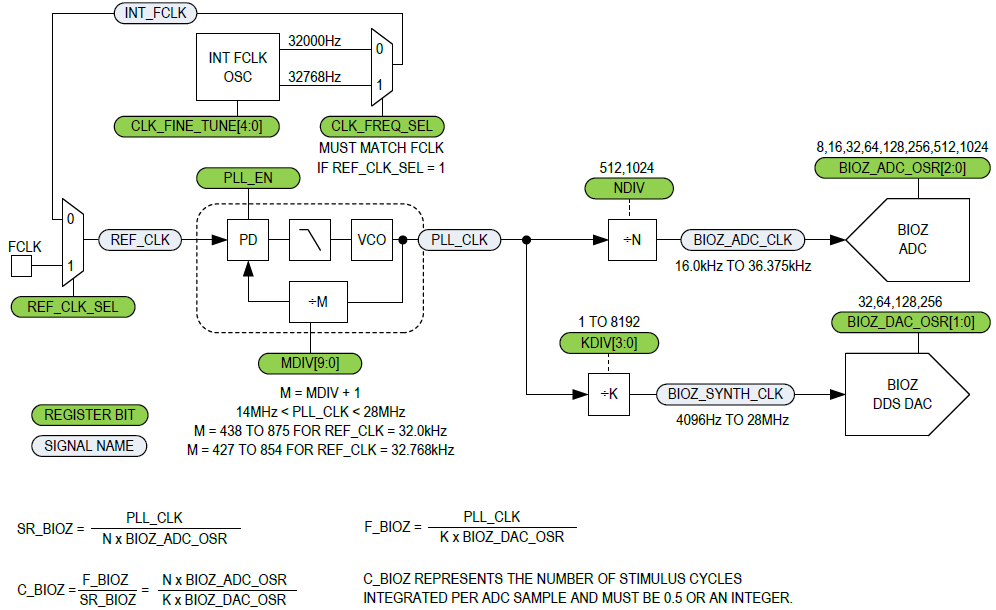
\includegraphics[width=1\textwidth]{Figures/max30009_clock.png} 
    \caption{Vremenski podsustav MAX30009 sustava \cite{max30009_datasheet}}
    \label{slk:max_30009_clock}
\end{figure}

Na slici \ref{slk:max_30009_clock} prikazan je vremenski podsustav MAX30009 integriranog sučelja za mjerenje bioimppedancije.
Kao početni takt sustava odabran je interni oscilator frekvencije 32.768 kHz. Taj se takt dalje vodi na umnoživač frekvencije 
(engl. \textit{PLL, phase-lock loop}) iz kojeg se dobivaju frekvencije između 14 i 28 MHz, u ovisnosti o konstanti MDIV. 
Nakon toga se konstantama KDIV, NDIV, 
BIOZ\_ADC\_OSR i BIOZ\_DAC\_OSR postavljaju frekvencija uzbudne struje i frekvencija uzorkovanja \cite{max30009_datasheet}.   

Pošto je glavna karakteristika sustava mjerenje bioimpedancije na različitim frekvencijama, upravljački program mora 
omogučavati brzu i laganu promjenu frekvencije uzbudne struje. Zbog toga je stvoren enumeracijki tip podataka koji 
sadrži popis svih korištenih frekvenija i omogućava pisanje generičkih funckija neovisnih o konkretnoj frekvenciji: 
\begin{lstlisting}[label={lst:enumeracija_frekvencija},style=CStyle,caption={Enumeracijski tip podataka za odabir frekvencije rada},captionpos=b]
typedef enum
{
    FREQ_5_kHz,
    FREQ_50_kHz,
    FREQ_100_kHz,
    FREQ_200_kHz,
    
    FREQ_CNT
} max30009_freq_t;
\end{lstlisting} 

Kako bi se promjenila frekvencija sustava potrebno je podesiti ranije spomenute konstante. 
Konstante su upisane u flash memoriju sustava u obliku polja vrijednosti točnim redosljedom kao 
u enumeracijskom tipu podataka za popis korištenih frekvencija što omogučava jednostavnu funkciju 
za promjenu frekvencije prikazanu u odsječku koda \ref{lst:promjena_frekvencije}. 

\begin{lstlisting}[label={lst:promjena_frekvencije},style=CStyle,caption={Funkcija za promjenu frekvenciju sustava},captionpos=b]
void max30009_change_freq(max30009_freq_t freq)
{
    // set dac_osr and adc_osr
    spi_api_change_reg(0x20, dac_osr[freq], 7, 2);
    spi_api_change_reg(0x20, adc_osr[freq], 5, 3);

    // set k,n
    spi_api_change_reg(0x17, k_div[freq], 4, 4);
    spi_api_change_reg(0x17, n_div[freq], 5, 1);

    //set m constant
    spi_api_change_reg(0x17, m_div[freq] & 0x300, 7, 2);         
    spi_api_write_reg(0x18, m_div[freq] & 0xFF);
}
\end{lstlisting}

Kalibracija sustava pokreče se na početku rada te traje nekoliko sekundi.
Za kalibraciju sustava koristi se vanjski precizni otpornik (napisi tu tocne specifikacije). 
Prije početka kalibracije sustav je potrebno konfigurirati na način da na mjerni kanal budu spojeni 
vanjski kalibracijski pinovi na koji je spojen kalibracijski otpornik. 
Kalibracija se provodi zasebno na svakoj frekvenciji rada sustava, te se kalibracijske konstante pohranjuju 
u memoriju sustava i kasnije koriste za korekciju rezultata mjerenja. 

Za kontrolu MAX30009 senzora stvorena je zasebna dretva. Na početku rada sustava vrši se početna inicijalizacija te 
kalibracija sustava. Nakon toga sustav je spreman za kontinuirano mjerenje. Mjerenje se pokreče i zaustavlja iz 
glavnog programa dvjema funkcijama koje prekidaju i ponovno pokreču dretvu:
\begin{lstlisting}[label={lst:max30009_kontrola},style=CStyle,caption={Funkcije za početak i prekid mjerenja},captionpos=b]
void max30009_start_measuring();
void max30009_stop_measuring();
\end{lstlisting}
U normalnom radu sustava dretva prolazi po svim frekvencijama navedenim u ranije opisanom enumeracijskom tipu podataka. 
Za svaku frekvenciju sustav je potrebno nanovo konfigurirati te pričekati da se sustav utitra na novoj frekvenciji rada. 
Radi toga nakon svake promjene frekvencije prva 3 očitanja su ignorirana i kao rezultat mjerenja uzima se četvrto očitanje. 
Izmjerni podatak ispravlja se u ovisnosti o kalibracijskim konstantama te se nakon toga šalje ispitnom okruženju BLE protokolom. 
Točan format slanja podataka bit će opisan u daljenjem tekstu.

- kak su podaci upisani i kak se dode do impedancije? to radije u onaj uvodni dio o senzoru ubacit

\section{Bluetooth low energy komunikacija}

Bluetooth Low Energy (BLE) je bežični komunikacijski protokol koji se često koristi u 
nosivim biomedicinskim uređajima zbog svoje energetske učinkovitosti i sposobnosti za prijenos podataka s malom potrošnjom energije.
Mala potrošnja od velike je važnosti kod nosivih uređaja jer time mogu imati manju bateriju i biti lakši te raditi dulje vremensko razdoblje 
bez punjenja ili zamjene baterije.

- neka slikica

BLE komunikacija odvija se s pomoću servisa i karakteristika. Servisi u BLE protokolu predstavljaju skupine funkcionalnosti koje 
uređaj može pružiti ili koristiti. Svaki servis ima jednu ili više karakteristika koje predstavljaju konkretne podatke ili operacije koje 
se mogu izvršiti.

Razvijeni nosivi sustav konfiguriran je kao Generic ATTribute Profile (GATT) server te pruža jedan servis imena \texttt{BodyFluidMonitoring}. 
Servis \texttt{BodyFluidMonitoring} sastoji se od dvije karakteristike, \texttt{ReceiveCommand} za primanje naredbi i 
\texttt{SendData} za slanje izmjerenih podataka ispitnom okruženju.

\begin{figure}[htb]
    \centering
    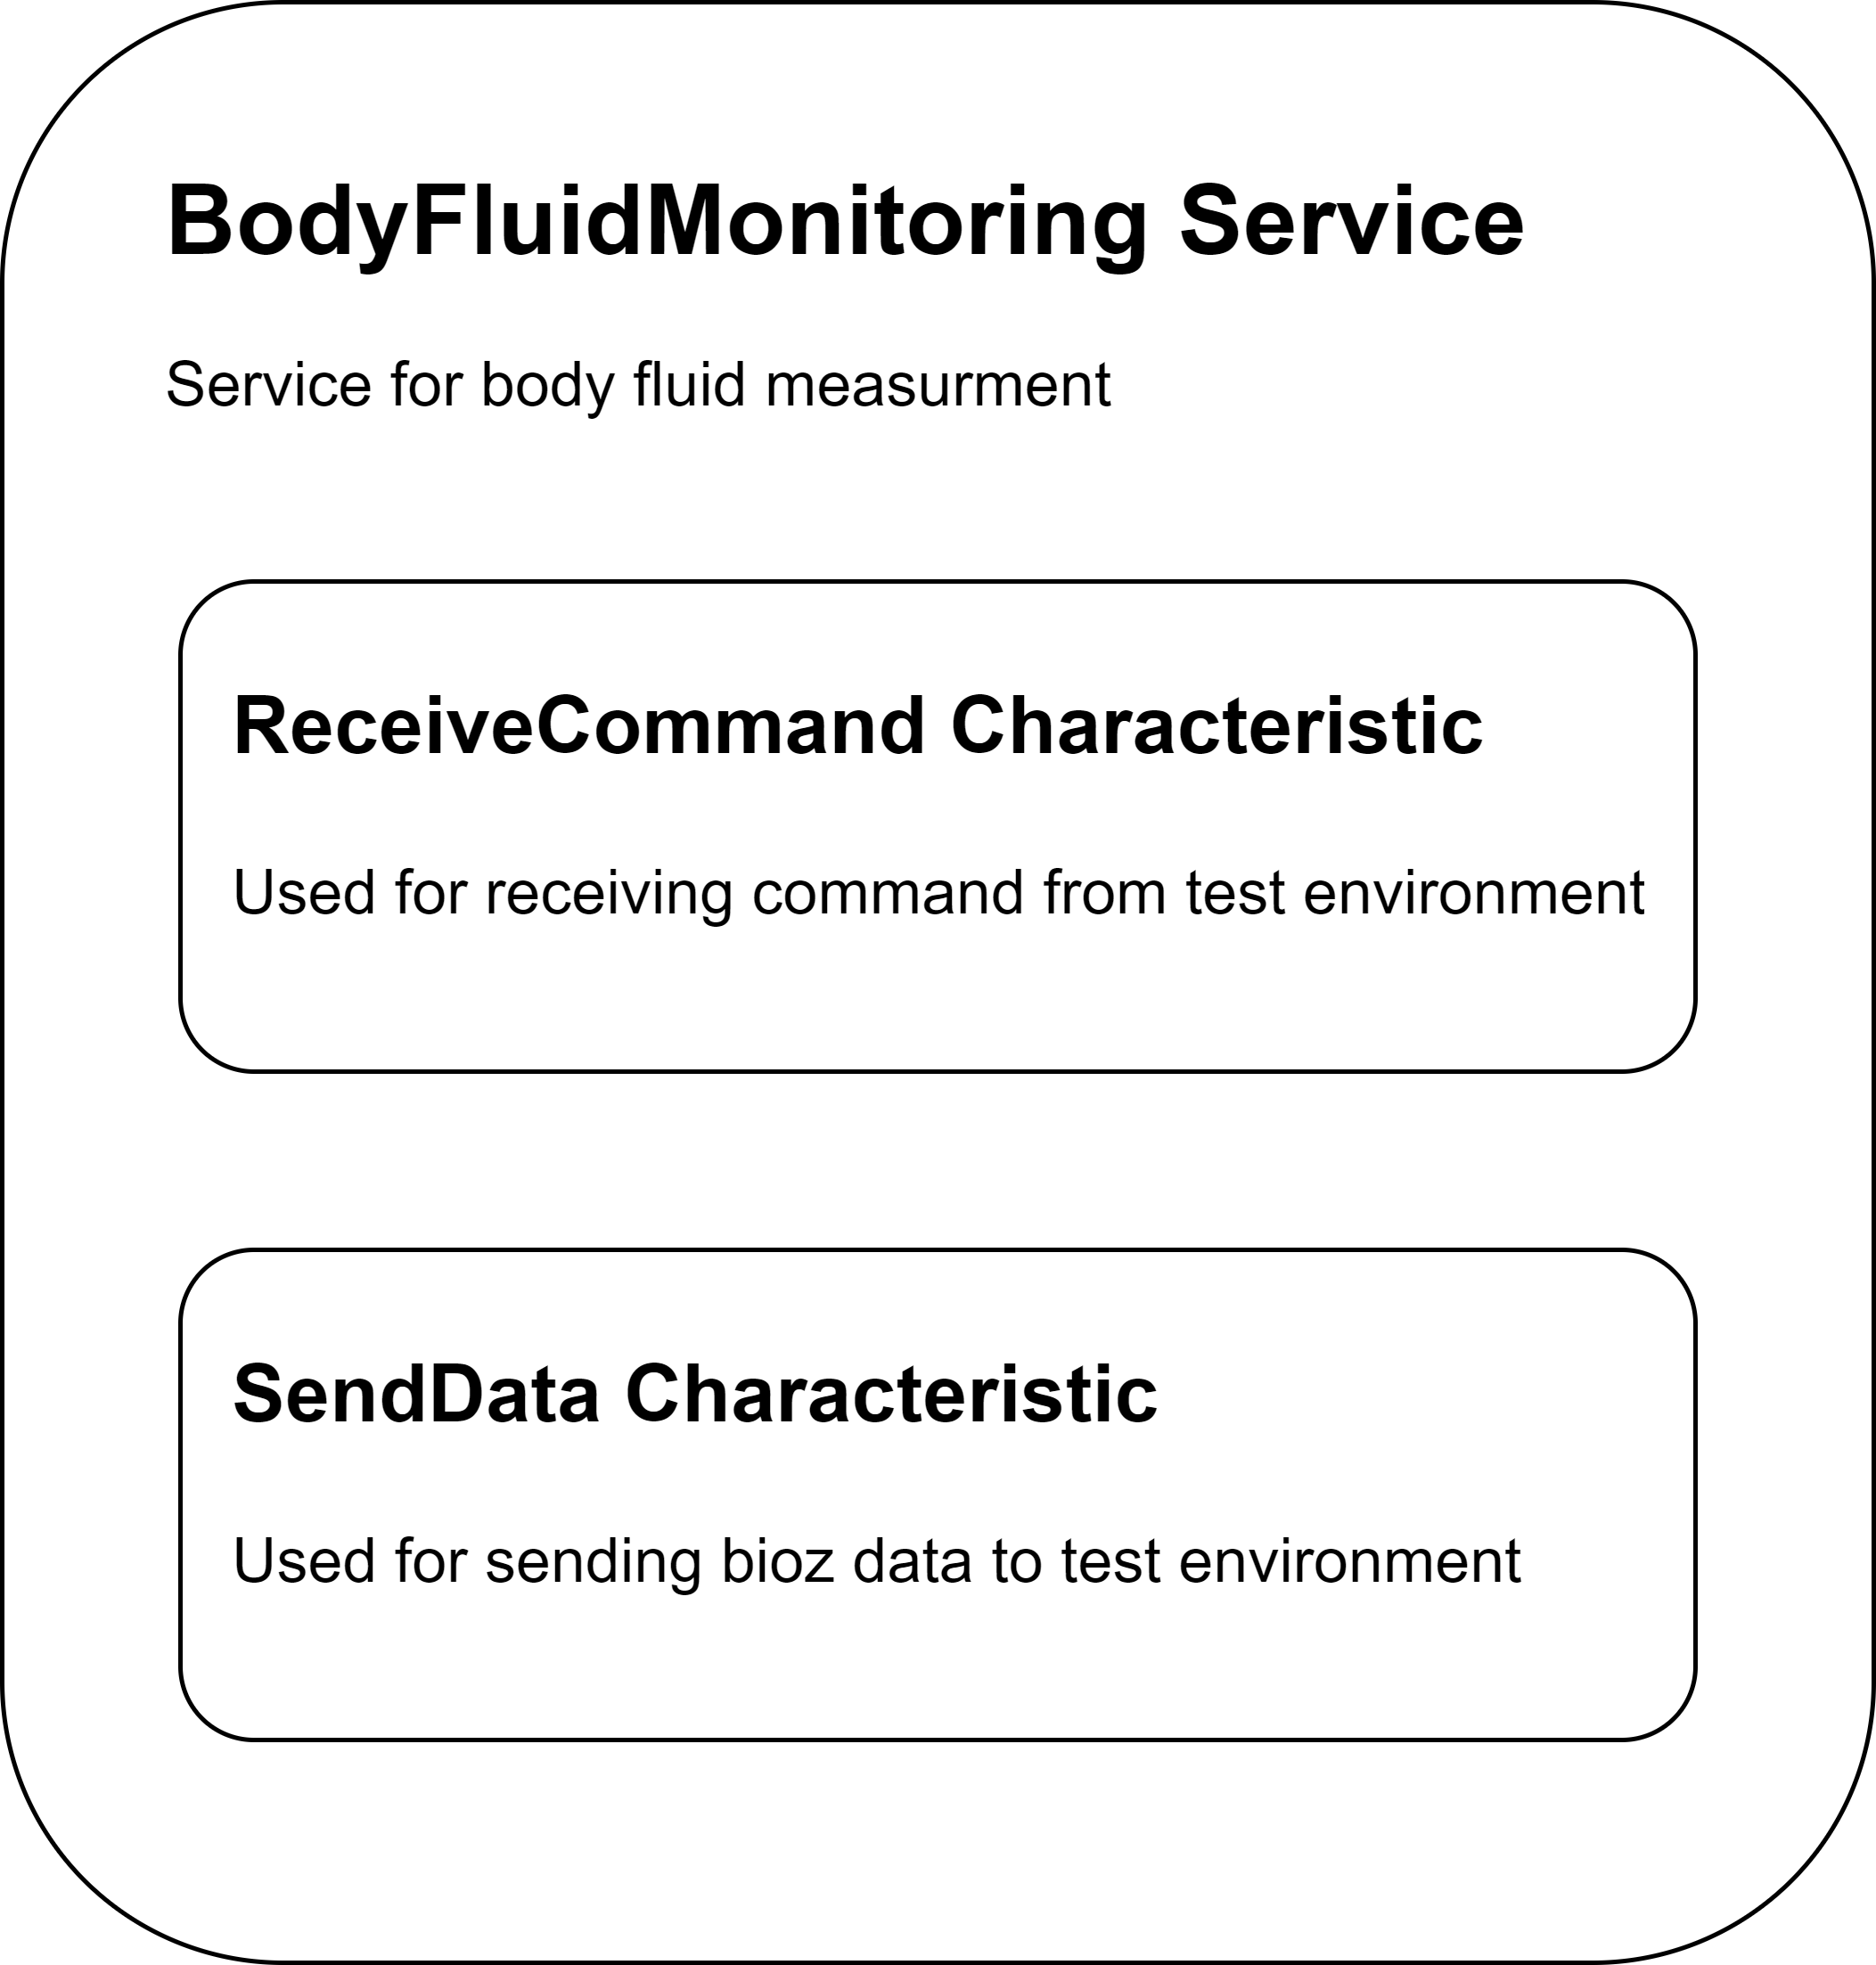
\includegraphics[width=0.5\textwidth]{Figures/ble_service.png} 
    \caption{Konfiguracija GATT servera}
    \label{slk:max_30009_clock}
\end{figure}

Razvijeno aplikacijsko programsko sučelje za kontrolu BLE komunikacije sastoji se od dvije funkcije:
\begin{lstlisting}[label={lst:ble_api},style=CStyle,caption={Programsko sučelje za kontrolu BLE komunikacije},captionpos=b]
void ble_send_data(void *data_to_send, uint8_t data_len);
void ble_init(void (*ble_cmd_handler_callback)(uint8_t));
\end{lstlisting} 

Funkcija \texttt{ble\_init(void (*ble\_cmd\_handler\_callback)(uint8\_t))} inicijalizira BLE periferiju te 
postavlja pokazivač na funkciju koja se poziva kada  \texttt{ReceiveCommand} karakteristika primi naredbu. 
Naredbe su kodirane kao cijeli brojevi te u sustavu postoje dvije, BLE\_CMD\_START i BLE\_CMD\_STOP, kojima se pokreče i zaustavlja mjerenje.  
\begin{lstlisting}[label={lst:ble_received_cmd},style=CStyle,caption={Funkcija koja se poziva kada je primljena naredba},captionpos=b]
static void receive_cmd(uint8_t val)
{
    if(BLE_CMD_START == val)
    {
        max30009_start_measuring();
    }
    else if(BLE_CMD_STOP == val)
    {
        max30009_stop_measuring();
    }
}
\end{lstlisting} 

Razvijeni sustav podatke ispitnom okruženju šalje funkcijom \texttt{ble\_send\_data(void *data\_to\_send, uint8\_t data\_len)} 
kojoj se prosljeđuje pokazivač na podatke koji se šalju i duljinu podataka za slanje. 
Izvršavanjem navedene funkcije ažurira se vrijednost karakteristike \texttt{SendData}.

-slikica ovog

Poruke se šalju u obliku niza znakova u formatu \texttt{vrijeme;senzor;podatci}. Format podataka ovisi o senzoru čiji se podatci šalju te je zbog toga uveden dodatan sloj 
apstrakcije između aplikacije i BLE komunikacijskog sučelja.
\begin{lstlisting}[label={lst:ble_send_sensor_data},style=CStyle,caption={Funkcija za slanje rezultata mjerenja sa pojedinog senzora},captionpos=b]
void ble_api_send_sensor_data(void *data_structure, sensor_t sensor);
\end{lstlisting} 
Pri pozivu funkcije za slanje podataka (\ref{lst:ble_send_sensor_data}) kao parametri se zadaju 
pokazivač na podatke senzora i enumeracijski tip \texttt{sensor\_t} koji određuje o kojem senzoru je riječ.
Funkcija dalje u ovisnosti o senzoru priprema niz znakova za slanje te poziva ranije opisane funckije BLE komunikacijskog sučelja 
(\ref{lst:ble_api}).

-primjer poruke? yes, no, maybe, I don't know.. can you repeat the question

\end{document}